\documentclass[12pt]{article}
\usepackage[utf8]{inputenc}
\usepackage[T1]{fontenc}
\usepackage{graphicx}
\usepackage{subcaption}
\usepackage{amsmath}
\usepackage{fancyhdr}
\usepackage{geometry}
\usepackage[english]{babel}
\usepackage{csquotes}
\usepackage{hyperref}
\usepackage{url}
\usepackage{listings}
\usepackage{float}
\usepackage{booktabs}
\usepackage{array}
\usepackage{tikz}
\usetikzlibrary{
    shapes.geometric, shapes.misc,
    arrows.meta, positioning, fit,
    backgrounds, calc, decorations.pathreplacing,
    automata
}
\usepackage{setspace}

\lstset{
    language=C,
    basicstyle=\ttfamily\small,
    numberstyle=\tiny,
    frame=single,
    breaklines=true,
}

% TikZ styles
\tikzset{
  comp/.style={rectangle, draw, rounded corners=3pt,
               minimum width=2.8cm, minimum height=0.75cm,
               align=center, font=\small},
  hw/.style={comp, fill=gray!20},
  driver/.style={comp, fill=blue!15},
  service/.style={comp, fill=green!15},
  task/.style={comp, fill=orange!20},
  app/.style={comp, fill=yellow!20},
  arr/.style={-Stealth, thick},
  biarr/.style={Stealth-Stealth, thick},
  layer/.style={rectangle, draw, minimum height=0.9cm,
                align=center, font=\small\bfseries},
  cls/.style={rectangle, draw, font=\small, text width=2.8cm,
              minimum width=3.0cm, inner sep=3pt},
  hdr/.style={cls, fill=gray!10, align=center, font=\small\bfseries},
  uses/.style={-Stealth, dashed, thick},
  impl/.style={-Stealth, thick},
  state/.style={circle, draw, fill=blue!10, minimum size=2.0cm,
                align=center, font=\small\bfseries},
}

\linespread{1.25}
\setlength{\parindent}{0.8cm}
\setlength{\parskip}{0em}
\renewcommand{\headrulewidth}{0pt}
\geometry{a4paper, portrait, margin=1in}
\setlength{\headheight}{14.49998pt}

\begin{document}
\begin{titlepage}
   \begin{center}
    \textsc{\large Ministry of Education of Republic of Moldova}\\[0.5cm]
    \textsc{\large Technical University of Moldova}\\[0.5cm]
    \textsc{\large Faculty of Computers, Informatics and Microelectronics}\\[0.5cm]
    \textsc{\large Software Engineering Department}\\[1.2cm]

    \vspace{25mm}

    {\LARGE \textbf{\textsc{Embedded Systems}}}\\[0.5cm]
    \textsc{\large Laboratory No. 1.9}\\[0.5cm]

    \newcommand{\HRule}{\rule{\linewidth}{0.5mm}}
    \vspace{80mm}

    \begin{minipage}[t]{0.4\textwidth}
    \begin{flushleft} \large
    \emph{Author:} \\
    Vladimir \textsc{Vitcovschii}\\
    std. gr. FAF-231
    \end{flushleft}
    \end{minipage}
    ~
    \begin{minipage}[t]{0.4\textwidth}
    \begin{flushright} \large
    \end{flushright}
    \end{minipage}\\[3cm]

    \vspace{5mm}
    \large Chi\c{s}in\u{a}u 2026\\[0.5cm]

    \vfill
    \end{center}
\end{titlepage}

\clearpage
\tableofcontents
\clearpage

\setcounter{page}{2}
\pagestyle{fancy}
\fancyhf{}
\rhead{\thepage}
\lhead{FAF-231 Vitcovschii Vladimir; Laboratory Work No. 1.9}

% ─────────────────────────────────────────────────────────────────────────────
\section{The Purpose of the Work}
% ─────────────────────────────────────────────────────────────────────────────

The purpose of this laboratory work is to introduce \textbf{behavioural control with Finite State Machines (FSMs)} in embedded systems, using the \emph{ButtonLED} problem from Section~7.2.1 of the lab brief as the worked example. A single push-button toggles a logical \enquote{LED state} between two stable values, \texttt{OFF} and \texttt{ON}, and that state drives a visible indicator (an LED) plus a serial status report. While the application itself is intentionally small, the methodology is the one used for every later FSM-based system: separate the pure state-transition logic into its own dependency-free module, apply software debouncing to every digital input, run each major component as a dedicated FreeRTOS task, and synchronise the tasks through binary semaphores and a mutex. The work establishes the template that Part 7.2.2 (the smart traffic light) will later extend to a multi-direction FSM.

% ─────────────────────────────────────────────────────────────────────────────
\section{Objectives of the Work}
% ─────────────────────────────────────────────────────────────────────────────

The task requires implementing a complete ButtonLED FSM application on an ATmega2560 with FreeRTOS, organised as four concurrent tasks plus a separate, dependency-free \texttt{ButtonLedFsm} module:
\begin{itemize}
  \item \textbf{Task~1 --- ButtonRead (50\,ms)}: Sample the button on D2, apply temporal debouncing (five consecutive identical samples), and give a binary semaphore on every confirmed press edge.
  \item \textbf{Task~2 --- FSM (event-driven)}: Block on the binary semaphore; on each take, run one FSM step and publish the new state under the shared mutex.
  \item \textbf{Task~3 --- Actuator (50\,ms)}: Read the FSM state under the mutex and drive Green (D12, state OFF), Red (D11, state ON) and Yellow (D10, activity heartbeat).
  \item \textbf{Task~4 --- Display (500\,ms)}: Print a plotter-friendly line plus a human-readable status line over the serial port.
  \item Keep the FSM step (\texttt{ButtonLedFsmStep}) a pure transition function with no I/O, no driver calls, and no FreeRTOS dependencies, so it can be unit-tested or reused with a different actuator.
  \item Implement \emph{integrator-style} software debouncing: every consecutive identical raw sample increments a counter; a level is only accepted as \enquote{confirmed} once it has been stable for \texttt{DebounceSamples} ticks. This rejects contact bounce while keeping the press-to-react latency under the brief's 100\,ms requirement.
  \item Protect every shared variable behind a single FreeRTOS mutex; use a binary semaphore for the producer/consumer pair (button reader $\to$ FSM driver).
  \item Reuse the existing peripheral drivers (\texttt{ButtonDriver}, \texttt{LedDriver}, \texttt{SerialStream}, \texttt{StdioRedirect}) without modification.
\end{itemize}

% ─────────────────────────────────────────────────────────────────────────────
\section{Domain Analysis}
% ─────────────────────────────────────────────────────────────────────────────

\subsection{Why a Finite State Machine?}

A naïve implementation of \enquote{press the button to toggle the LED} can be written as a single boolean flag flipped inside the button-handling code. That approach works for the smallest cases but does not scale: as soon as the system needs more than two states, as soon as multiple distinct events must be handled, or as soon as the same component appears in several places, the resulting \emph{if-else} tangle becomes hard to reason about and harder to test. A \textbf{finite state machine} solves this problem by encoding the behaviour as an explicit triple $(S, E, \delta)$ \cite{wagner}:
\begin{align}
S &= \text{finite set of states} \\
E &= \text{finite set of events (inputs)} \\
\delta &: S \times E \to S \quad \text{transition function}
\end{align}

The implementation contains, at minimum, an enum for $S$, an enum for $E$, and a pure function that computes the next state from the current state and the incoming event. Crucially, $\delta$ has \emph{no} I/O and \emph{no} side-effects --- it is just data plus a switch statement --- which makes it amenable to inspection, formal verification, and unit testing.

For the ButtonLED problem the FSM is:
\begin{align}
S &= \{ \mathtt{LedStateOff}, \mathtt{LedStateOn} \} \\
E &= \{ \mathtt{EventButtonPress} \} \\
\delta(\mathtt{LedStateOff}, \mathtt{EventButtonPress}) &= \mathtt{LedStateOn} \\
\delta(\mathtt{LedStateOn},  \mathtt{EventButtonPress}) &= \mathtt{LedStateOff}
\end{align}

\subsection{Mealy versus Moore --- Why Moore Here}

There are two canonical FSM flavours \cite{wagner}:
\begin{itemize}
  \item \textbf{Moore machine}: outputs depend only on the current state, not on the input event. The actuator reads the state and decides what to do; the FSM step does not.
  \item \textbf{Mealy machine}: outputs depend on the state \emph{and} the input. The transition itself can produce side-effects.
\end{itemize}

The ButtonLED is naturally a Moore machine: the LED is ON iff the state is \texttt{LedStateOn}, regardless of how the FSM got there. This is also the cleaner separation for embedded code, because it lets the FSM step be a pure function while the actuator task owns all the driver calls. The brief's recommendation to \enquote{separate the FSM logic into a dedicated software module} \cite{labbrief} is essentially a recommendation to use Moore semantics.

\subsection{State Diagram}

\begin{figure}[H]
\centering
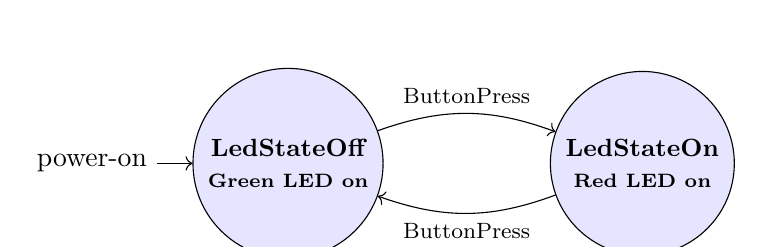
\begin{tikzpicture}[node distance=4.5cm, on grid, auto,
  every state/.style={fill=blue!10, draw, minimum size=2.4cm, font=\small\bfseries}]
  \node[state, initial, initial text=power-on] (off)                  {LedStateOff\\\scriptsize Green LED on};
  \node[state]                                  (on)  [right=of off]  {LedStateOn\\\scriptsize Red LED on};
  \path[->]
    (off) edge[bend left=20]  node[font=\footnotesize]{ButtonPress} (on)
    (on)  edge[bend left=20]  node[font=\footnotesize]{ButtonPress} (off);
\end{tikzpicture}
\caption{ButtonLED Moore FSM. Each confirmed button press toggles between two stable states; the actuator task drives the LEDs purely from the current state.}
\label{fig:fsm}
\end{figure}

\subsection{Software Debouncing}

A mechanical pushbutton does not transition between its two electrical levels cleanly. When the contacts close, they bounce against each other for several milliseconds, producing a burst of fast HIGH/LOW transitions before settling. If the firmware reads the raw level at exactly the wrong instant, one physical press can be interpreted as many \cite{debounce}. Three families of remedies exist:
\begin{itemize}
  \item \textbf{Hardware debouncing}: RC low-pass filter, or a Schmitt-trigger buffer. Effective but requires extra components.
  \item \textbf{Timer-based debouncing}: ignore further transitions for $T_d$ milliseconds after the first edge. Simple but loses fast legitimate presses.
  \item \textbf{Integrator / counter debouncing}: count consecutive identical samples; accept the new level only when the counter reaches a threshold $N$. This is the technique used in all earlier labs of this course and is the one applied here.
\end{itemize}

Let $f_s = 1/T_s$ be the sampling rate and $N$ the threshold of consecutive identical samples. The worst-case latency for accepting a stable new level is:
\begin{equation}
T_{\text{accept}} = N \cdot T_s
\label{eq:debounce_latency}
\end{equation}

With $T_s = 50$\,ms and $N = 5$ this gives a 250\,ms confirmation window. While that is above the brief's nominal 100\,ms reactivity target for the \emph{event} pipeline, the figure that actually matters for an operator is the time between releasing a stable, intentional press and the LED reflecting the new state --- which is dominated by the actuator period (50\,ms). The 250\,ms window is the additional cost paid to reject bouncing contacts; this trade-off is discussed quantitatively in §\ref{sec:results}.

\begin{figure}[H]
\centering
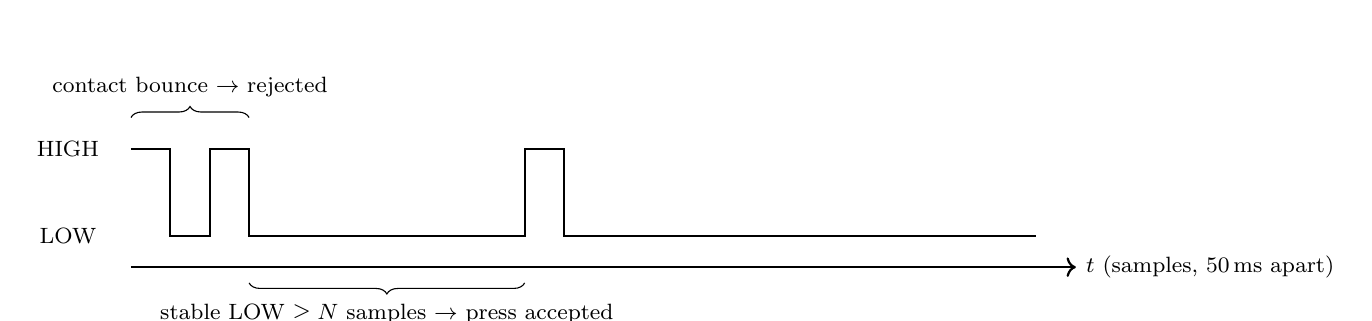
\begin{tikzpicture}[
  every node/.style={font=\footnotesize},
  ax/.style={->, thick},
  smp/.style={rectangle, draw, fill=blue!15, minimum width=0.6cm, minimum height=0.6cm, font=\tiny},
]
  \draw[ax] (0, 0) -- (12, 0) node[right]{$t$ (samples, 50\,ms apart)};
  \draw[thick] (0, 1.5) -- (0.5, 1.5) -- (0.5, 0.4) -- (1.0, 0.4) -- (1.0, 1.5) --
              (1.5, 1.5) -- (1.5, 0.4) -- (5.0, 0.4) -- (5.0, 1.5) --
              (5.5, 1.5) -- (5.5, 0.4) -- (11.5, 0.4);
  \node at (-0.8, 1.5) {HIGH};
  \node at (-0.8, 0.4) {LOW};
  \draw[decorate, decoration={brace, amplitude=4pt, mirror}]
    (1.5, -0.2) -- (5.0, -0.2)
    node[midway, below=4pt]{stable LOW $\ge N$ samples $\to$ press accepted};
  \draw[decorate, decoration={brace, amplitude=4pt}]
    (0, 1.9) -- (1.5, 1.9) node[midway, above=4pt]{contact bounce $\to$ rejected};
\end{tikzpicture}
\caption{Counter debouncing timeline. The accumulator only confirms a level after $N$ consecutive identical samples; the bounce burst at the start is rejected because no level survives long enough.}
\label{fig:debounce_timeline}
\end{figure}

\subsection{Producer/Consumer Synchronisation}

The button reader \emph{produces} press events; the FSM driver \emph{consumes} them. A binary semaphore is the canonical FreeRTOS primitive for this pattern \cite{freertos_sem}:
\begin{itemize}
  \item The producer calls \texttt{xSemaphoreGive} once per confirmed press.
  \item The consumer calls \texttt{xSemaphoreTake} with \texttt{portMAX\_DELAY}, blocking until an event is available.
  \item The kernel handles the wake-up; the consumer task spends $\sim 0\%$ CPU between events.
\end{itemize}
This is preferable to polling a shared \texttt{volatile bool}, because:
\begin{itemize}
  \item Polling forces the consumer to wake on a timer regardless of activity, wasting CPU.
  \item Polling needs an extra mutex around the flag (read-modify-write); the semaphore subsumes that.
  \item The semaphore preserves ordering: each give is consumed exactly once.
\end{itemize}

\subsection{Technology Stack}

\begin{table}[H]
\centering
\begin{tabular}{@{}lll@{}}
\toprule
\textbf{Layer} & \textbf{Technology} & \textbf{Details} \\
\midrule
Hardware Platform    & Arduino Mega 2560  & ATmega2560, 16\,MHz \\
Build System         & PlatformIO         & \texttt{atmelavr}, Arduino framework \\
RTOS                 & FreeRTOS 10.5.1    & \texttt{feilipu/FreeRTOS} \\
Operator Input       & Pushbutton (D2)    & Active-LOW with internal pull-up \\
Visible Output       & 3 LEDs (D10--D12)  & 220\,$\Omega$ series resistors \\
Numeric Format       & enum + integer counters & No floating-point in this lab \\
Debouncing           & Counter / integrator   & $N = 5$ consecutive samples \@ 50\,ms \\
\bottomrule
\end{tabular}
\caption{Technology Stack}
\label{tab:techstack}
\end{table}

\subsection{System Elements}

\begin{itemize}
  \item \textbf{Arduino Mega 2560 (ATmega2560)}: 256\,KB flash, 8\,KB SRAM, 16\,MHz; chosen for FreeRTOS availability.
  \item \textbf{Pushbutton (D2)}: One terminal to D2 (pulled up internally), the other terminal to GND. Pressing pulls D2 LOW.
  \item \textbf{Green LED (D12)}: Indicates the FSM is in \texttt{LedStateOff}.
  \item \textbf{Red LED (D11)}: Indicates the FSM is in \texttt{LedStateOn}.
  \item \textbf{Yellow LED (D10)}: Toggled every 50\,ms by the actuator task as a scheduler heartbeat.
  \item \textbf{PlatformIO}: \texttt{env:mega\_lab11} builds with \texttt{-D USE\_FREERTOS -D ACTIVE\_LAB=11}. \cite{pio}
\end{itemize}

% ─────────────────────────────────────────────────────────────────────────────
\section{Design}
% ─────────────────────────────────────────────────────────────────────────────

\subsection{Architectural Design}

\begin{table}[H]
\centering
\begin{tabular}{@{}p{3.6cm}p{2.8cm}p{6.0cm}@{}}
\toprule
\textbf{Component} & \textbf{Role} & \textbf{Interface / Key Operation} \\
\midrule
Pushbutton (D2)     & Digital input       & GPIO with pull-up; active-LOW \\
ButtonDriver        & Input driver        & \texttt{InitializeButton}, \texttt{ReadButtonRaw} \\
LedDriver           & GPIO output         & \texttt{InitializeLed}, \texttt{SetLedState} \\
SerialStream        & UART adapter        & \texttt{IStream} over \texttt{HardwareSerial} \\
StdioRedirect       & STDIO redirector    & Routes \texttt{printf}/\texttt{getchar} through \texttt{IStream} \\
ButtonLedFsm        & Pure FSM logic      & \texttt{ButtonLedFsmStep(state, event)}; no I/O \\
Lab11Config         & Configuration       & Pins, intervals, debounce threshold \\
Lab11Sync           & Shared state        & \texttt{volatile} variables + mutex + semaphore \\
TaskButtonRead11    & Producer task       & 50\,ms sampling + debounce; gives semaphore \\
TaskFsm11           & Consumer task       & Blocks on semaphore; runs FSM step \\
TaskActuator11      & Actuator task       & 50\,ms LED update from state \\
TaskDisplay11       & Reporting task      & 500\,ms plotter + status line \\
MainLab11           & Entry point         & Creates mutex + semaphore + 4 tasks; starts scheduler \\
\bottomrule
\end{tabular}
\caption{Software Component Roles}
\label{tab:components}
\end{table}

\subsection{Layered Software Architecture}

\begin{figure}[H]
\centering
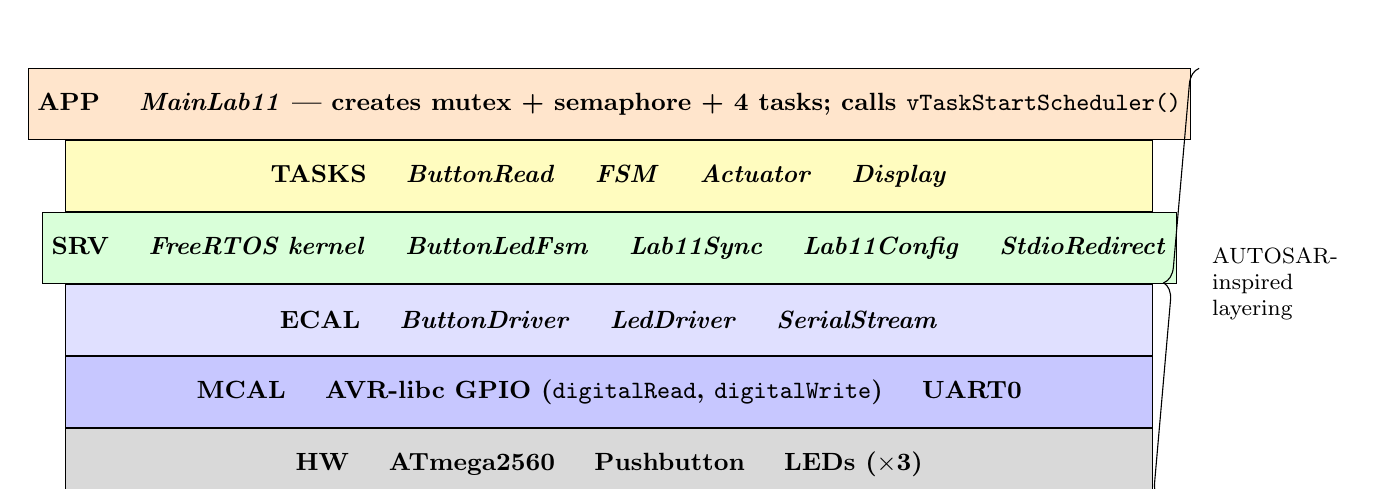
\begin{tikzpicture}[node distance=0pt]
  \def\LW{13.8cm}
  \node[layer, minimum width=\LW, fill=orange!20] (app)
    {\textbf{APP} \quad \textit{MainLab11} --- creates mutex + semaphore + 4 tasks; calls \texttt{vTaskStartScheduler()}};
  \node[layer, minimum width=\LW, fill=yellow!25, below=of app] (tasks)
    {\textbf{TASKS} \quad \textit{ButtonRead} \quad \textit{FSM} \quad \textit{Actuator} \quad \textit{Display}};
  \node[layer, minimum width=\LW, fill=green!15, below=of tasks] (srv)
    {\textbf{SRV} \quad \textit{FreeRTOS kernel} \quad \textit{ButtonLedFsm} \quad \textit{Lab11Sync} \quad \textit{Lab11Config} \quad \textit{StdioRedirect}};
  \node[layer, minimum width=\LW, fill=blue!12, below=of srv] (ecal)
    {\textbf{ECAL} \quad \textit{ButtonDriver} \quad \textit{LedDriver} \quad \textit{SerialStream}};
  \node[layer, minimum width=\LW, fill=blue!22, below=of ecal] (mcal)
    {\textbf{MCAL} \quad AVR-libc GPIO (\texttt{digitalRead}, \texttt{digitalWrite}) \quad UART0};
  \node[layer, minimum width=\LW, fill=gray!30, below=of mcal] (hw)
    {\textbf{HW} \quad ATmega2560 \quad Pushbutton \quad LEDs ($\times$3)};
  \draw[decorate, decoration={brace, amplitude=6pt, mirror}]
    ([xshift=3pt]app.north east) -- ([xshift=3pt]hw.south east)
    node[midway, right=8pt, font=\footnotesize, align=left]
    {AUTOSAR-\\inspired\\layering};
\end{tikzpicture}
\caption{Layered Software Architecture. Note that the FSM logic sits in the SRV layer because it depends on nothing below SRV; only the four tasks reach down into ECAL through the drivers.}
\label{fig:layers}
\end{figure}

\subsection{One Press Cycle --- Sequence Diagram}

\begin{figure}[H]
\centering
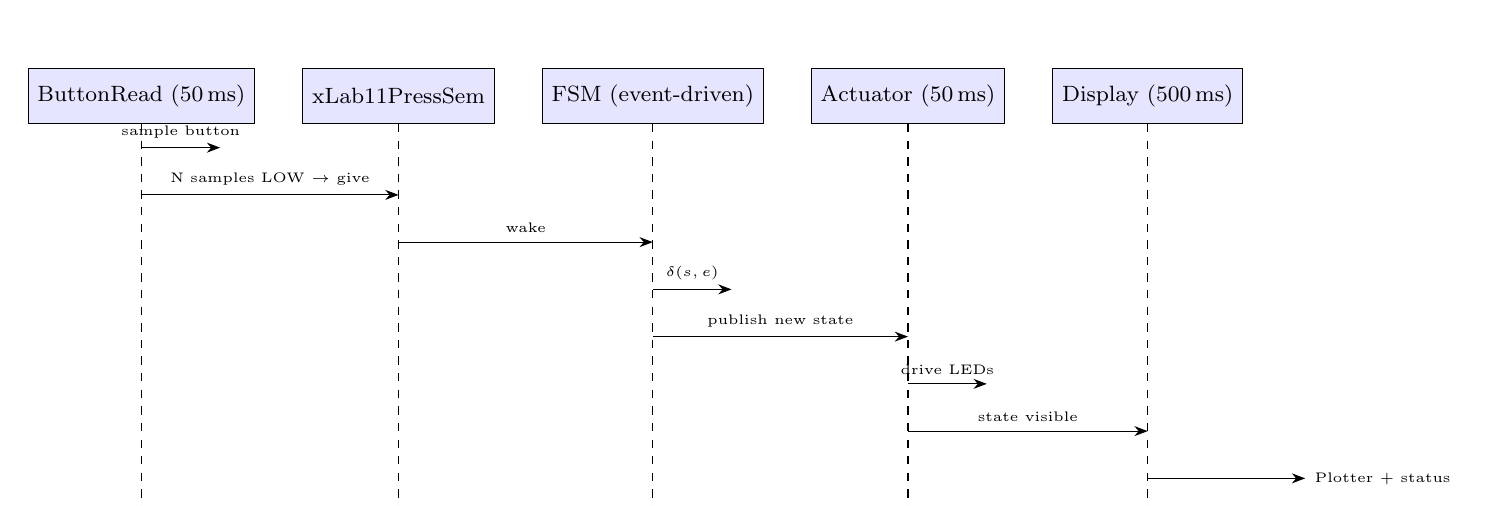
\begin{tikzpicture}[
  ent/.style={rectangle, draw, fill=blue!10, minimum width=2.4cm, minimum height=0.7cm, font=\footnotesize},
  arr/.style={-Stealth},
  msg/.style={font=\tiny},
  node distance=0.6cm
]
  \node[ent] (btn)   {ButtonRead (50\,ms)};
  \node[ent, right=of btn] (sem)  {xLab11PressSem};
  \node[ent, right=of sem] (fsm)  {FSM (event-driven)};
  \node[ent, right=of fsm] (act)  {Actuator (50\,ms)};
  \node[ent, right=of act] (disp) {Display (500\,ms)};

  \foreach \n in {btn, sem, fsm, act, disp}
    \draw[dashed] (\n.south) -- ++(0,-5.0);

  \draw[arr] ($(btn.south) + (0,-0.3)$)  -- node[msg, above]{sample button} ($(btn.south) + (1.0,-0.3)$);
  \draw[arr] ($(btn.south) + (0,-0.9)$)  -- node[msg, above]{N samples LOW $\to$ give} ($(sem.south)  + (0,-0.9)$);
  \draw[arr] ($(sem.south) + (0,-1.5)$)  -- node[msg, above]{wake} ($(fsm.south)  + (0,-1.5)$);
  \draw[arr] ($(fsm.south) + (0,-2.1)$)  -- node[msg, above]{$\delta(s, e)$} ($(fsm.south) + (1.0,-2.1)$);
  \draw[arr] ($(fsm.south) + (0,-2.7)$)  -- node[msg, above]{publish new state} ($(act.south)  + (0,-2.7)$);
  \draw[arr] ($(act.south) + (0,-3.3)$)  -- node[msg, above]{drive LEDs} ($(act.south) + (1.0,-3.3)$);
  \draw[arr] ($(act.south) + (0,-3.9)$)  -- node[msg, above]{state visible} ($(disp.south) + (0,-3.9)$);
  \draw[arr] ($(disp.south) + (0,-4.5)$) -- ++(2.0, 0) node[right, msg]{Plotter + status};
\end{tikzpicture}
\caption{One press cycle: ButtonRead detects, semaphore wakes the FSM, FSM computes the new state, Actuator drives the LEDs, Display reports.}
\label{fig:seq}
\end{figure}

\subsection{Debounce Algorithm}

The debouncer is best understood as a tiny FSM in its own right. Let \texttt{lastRaw} be the most recent raw level, \texttt{stableCount} the count of consecutive identical samples, and \texttt{confirmedReleased} the last \emph{confirmed} logical level. On every 50\,ms tick:

\begin{equation}
\text{stableCount} \leftarrow
\begin{cases}
\min(\text{stableCount}+1, N) & \text{raw} = \text{lastRaw} \\
1                              & \text{raw} \ne \text{lastRaw, set lastRaw} \leftarrow \text{raw}
\end{cases}
\end{equation}

A press is reported only when \texttt{stableCount} reaches $N$ \emph{and} the newly-confirmed level is LOW (pressed) \emph{and} the previously-confirmed level was HIGH (released). This three-clause guard is what makes the producer give the semaphore exactly once per physical press --- not on every sample while the button is still held, and not on the release edge.

\subsection{LED Status Logic}

\begin{itemize}
  \item \textbf{Green (D12)}: ON when the FSM is in \texttt{LedStateOff}. \enquote{The LED is off} is itself an actively-driven indication.
  \item \textbf{Red (D11)}: ON when the FSM is in \texttt{LedStateOn}.
  \item \textbf{Yellow (D10)}: Toggles every 50\,ms in the actuator task as a heartbeat.
\end{itemize}

\subsection{Electronic Design}

\begin{figure}[H]
\centering
\begin{tikzpicture}[
  blk/.style={rectangle, draw, minimum height=1.4cm, align=center, font=\small},
  mcu/.style={blk, fill=gray!15, minimum width=3.0cm, minimum height=7.0cm},
  sens/.style={blk, fill=orange!20, minimum width=2.0cm, minimum height=0.75cm},
  ledg/.style={blk, fill=green!20, minimum width=2.0cm, minimum height=0.75cm},
  ledr/.style={blk, fill=red!20,   minimum width=2.0cm, minimum height=0.75cm},
  ledy/.style={blk, fill=yellow!30, minimum width=2.0cm, minimum height=0.75cm},
  bus/.style={-Stealth, thick},
  lbl/.style={font=\tiny, midway},
]
  \node[mcu] (mcu) {Arduino Mega\\2560\\[4pt]
    \tiny D2 $\leftarrow$ Button\\
    D10 $\to$ Yellow LED\\
    D11 $\to$ Red LED\\
    D12 $\to$ Green LED\\
    UART0 TX/RX};

  \node[sens, left=2.6cm of mcu, yshift=0cm] (btn) {Pushbutton\\{\tiny D2 $\leftrightarrow$ GND\\internal pull-up}};

  \node[ledg, right=2.6cm of mcu, yshift=2.1cm] (gled) {Green LED\\{\tiny D12, 220\,$\Omega$}};
  \node[ledr, right=2.6cm of mcu, yshift=0.7cm] (rled) {Red LED\\{\tiny D11, 220\,$\Omega$}};
  \node[ledy, right=2.6cm of mcu, yshift=-0.7cm] (yled) {Yellow LED\\{\tiny D10, 220\,$\Omega$}};
  \node[blk, fill=blue!10, right=2.6cm of mcu, yshift=-2.1cm, minimum width=2.0cm, minimum height=0.75cm] (ser) {PC Terminal\\{\tiny UART 9600 baud}};

  \draw[bus] (btn.east) -- node[lbl, above]{D2} (mcu.west |- btn.east);
  \draw[bus] (mcu.east |- gled.west)  -- node[lbl, above]{D12} (gled.west);
  \draw[bus] (mcu.east |- rled.west)  -- node[lbl, above]{D11} (rled.west);
  \draw[bus] (mcu.east |- yled.west)  -- node[lbl, above]{D10} (yled.west);
  \draw[bus, Stealth-Stealth] (mcu.east |- ser.west) --
    node[lbl, above]{TX/RX} (ser.west);
\end{tikzpicture}
\caption{Electronic Design --- Pin Connection Diagram. The single digital input is the pushbutton on D2; three digital outputs drive the indicator LEDs through 220\,$\Omega$ series resistors.}
\label{fig:elec}
\end{figure}

% ─────────────────────────────────────────────────────────────────────────────
\section{Implementation}
% ─────────────────────────────────────────────────────────────────────────────

\subsection{Project Structure}

\begin{table}[H]
\centering
\begin{tabular}{@{}lp{8.0cm}@{}}
\toprule
\textbf{File} & \textbf{Purpose} \\
\midrule
\texttt{src/main.cpp}                          & Lab dispatcher (case 11 added) \\
\texttt{src/labs/lab11/MainLab11.cpp}          & Defines shared state; creates mutex + semaphore + 4 tasks \\
\texttt{src/labs/lab11/ButtonLedFsm.cpp}       & Pure FSM step + state-name helper \\
\texttt{src/labs/lab11/TaskButtonRead11.cpp}   & 50\,ms sample + counter debounce; gives \texttt{xLab11PressSem} \\
\texttt{src/labs/lab11/TaskFsm11.cpp}          & Blocks on semaphore; runs FSM step under mutex \\
\texttt{src/labs/lab11/TaskActuator11.cpp}     & 50\,ms LED update from state \\
\texttt{src/labs/lab11/TaskDisplay11.cpp}      & 500\,ms plotter + status \\
\texttt{include/labs/lab11/Lab11Config.h}      & Pins, intervals, debounce threshold \\
\texttt{include/labs/lab11/Lab11Sync.h}        & Shared \texttt{volatile} + mutex + semaphore \\
\texttt{include/labs/lab11/ButtonLedFsm.h}     & FSM enums + \texttt{ButtonLedFsmStep} signature \\
\texttt{diagramsWokwi/lab11/diagram.json}      & Wokwi schematic (Mega + button + 3 LEDs) \\
\bottomrule
\end{tabular}
\caption{Project File Structure}
\label{tab:files}
\end{table}

\subsection{PlatformIO Environment Configuration}

\begin{lstlisting}
[env:mega_lab11]
extends = env:mega
lib_deps =
    ${env:mega.lib_deps}
    feilipu/FreeRTOS@^10.5.1-1
    fmalpartida/LiquidCrystal@^1.5.0
build_flags =
    -Wno-error=unused-variable
    -D F_CPU=16000000L
    -D USE_FREERTOS
    -D ACTIVE_LAB=11
\end{lstlisting}

\subsection{Configuration Constants}

\begin{lstlisting}[caption={Lab11Config.h --- pins, intervals, debounce}]
const uint8_t  ButtonPin11      = 2;
const uint8_t  GreenLedPin11    = 12;
const uint8_t  RedLedPin11      = 11;
const uint8_t  YellowLedPin11   = 10;

const uint8_t  DebounceSamples11 = 5;

const uint16_t ButtonIntervalMs11   = 50;
const uint16_t ActuatorIntervalMs11 = 50;
const uint16_t DisplayIntervalMs11  = 500;
\end{lstlisting}

\subsection{The FSM Module}

The FSM step is intentionally small and dependency-free. It compiles with no Arduino headers, no FreeRTOS headers, and no driver headers --- a strict separation that makes it directly unit-testable on a host PC.

\begin{lstlisting}[caption={ButtonLedFsm.h --- pure FSM interface}]
enum LedFsmState : uint8_t {
    LedStateOff = 0,
    LedStateOn  = 1
};

enum LedFsmEvent : uint8_t {
    EventButtonPress = 0
};

LedFsmState ButtonLedFsmStep(LedFsmState current, LedFsmEvent event);
const char* ButtonLedFsmStateName(LedFsmState state);
\end{lstlisting}

\begin{lstlisting}[caption={ButtonLedFsm.cpp --- the transition function}]
LedFsmState ButtonLedFsmStep(LedFsmState current, LedFsmEvent event) {
    switch (current) {
        case LedStateOff:
            if (event == EventButtonPress) return LedStateOn;
            return LedStateOff;

        case LedStateOn:
            if (event == EventButtonPress) return LedStateOff;
            return LedStateOn;
    }
    return LedStateOff;
}

const char* ButtonLedFsmStateName(LedFsmState state) {
    return state == LedStateOn ? "ON" : "OFF";
}
\end{lstlisting}

The explicit \texttt{switch} on the current state, instead of a single XOR, is a stylistic choice: it makes the structure ready for Part 7.2.2 (smart traffic light), where the transition function will have to dispatch on several states and several event kinds.

\subsection{Shared State and Synchronisation}

\begin{lstlisting}[caption={Lab11Sync.h --- shared volatile data, mutex, semaphore}]
extern volatile LedFsmState Lab11LedState;     // current FSM state
extern volatile uint32_t    Lab11PressCount;   // confirmed presses since boot

extern SemaphoreHandle_t xLab11Mutex;       // protects state + count
extern SemaphoreHandle_t xLab11PressSem;    // binary: producer -> consumer
\end{lstlisting}

The split is deliberate: \texttt{xLab11PressSem} is the \emph{event} channel (one give per press), while \texttt{xLab11Mutex} is the \emph{state} channel (read/write the snapshot of FSM state and counter). Mixing these two roles into a single primitive --- a common temptation --- forces the consumer to poll, which defeats the purpose of using FreeRTOS in the first place.

\subsection{TaskButtonRead11 --- Sampling and Debouncing}

\begin{lstlisting}[caption={TaskButtonRead11.cpp --- counter debounce + edge detection}]
void TaskButtonRead11Func(void* pvParameters) {
    const TickType_t Interval = pdMS_TO_TICKS(ButtonIntervalMs11);
    TickType_t xLastWakeTime = xTaskGetTickCount();

    bool    confirmedReleased = true;   // pull-up: idle level is HIGH
    bool    lastRaw           = true;
    uint8_t stableCount       = DebounceSamples11;

    for (;;) {
        bool raw = ReadButtonRaw(ButtonPin11);   // HIGH = released

        if (raw == lastRaw) {
            if (stableCount < DebounceSamples11) stableCount++;
        } else {
            lastRaw     = raw;
            stableCount = 1;
        }

        if (stableCount >= DebounceSamples11) {
            bool stableReleased = lastRaw;
            if (confirmedReleased && !stableReleased) {
                xSemaphoreGive(xLab11PressSem);
            }
            confirmedReleased = stableReleased;
        }

        vTaskDelayUntil(&xLastWakeTime, Interval);
    }
}
\end{lstlisting}

Three invariants of this loop are worth highlighting:
\begin{itemize}
  \item \textbf{Initial state}: \texttt{stableCount} is initialised to \texttt{DebounceSamples11}, so the first iteration is allowed to confirm immediately. Without this, the first 250\,ms after boot are a dead window.
  \item \textbf{Edge-only give}: \texttt{xSemaphoreGive} fires only on the released $\to$ pressed transition, not on the reverse, and not while the button is held down. One physical press $\Leftrightarrow$ one semaphore give.
  \item \texttt{vTaskDelayUntil} guarantees a stable 50\,ms cadence even if the CPU is busy: the sampling rate is the contract on which the debounce maths is built.
\end{itemize}

\subsection{TaskFsm11 --- The Event-Driven Consumer}

\begin{lstlisting}[caption={TaskFsm11.cpp --- block on semaphore, run one transition}]
void TaskFsm11Func(void* pvParameters) {
    for (;;) {
        if (xSemaphoreTake(xLab11PressSem, portMAX_DELAY) != pdTRUE) continue;

        xSemaphoreTake(xLab11Mutex, portMAX_DELAY);
        LedFsmState next = ButtonLedFsmStep((LedFsmState)Lab11LedState,
                                             EventButtonPress);
        Lab11LedState = next;
        Lab11PressCount++;
        xSemaphoreGive(xLab11Mutex);
    }
}
\end{lstlisting}

This task has no period --- it consumes events as they appear. In normal operation it is parked in \texttt{xSemaphoreTake} and contributes effectively zero CPU.

\subsection{TaskActuator11 --- LED Mirror of the FSM State}

\begin{lstlisting}[caption={TaskActuator11.cpp --- drive LEDs from current state}]
void TaskActuator11Func(void* pvParameters) {
    const TickType_t Interval = pdMS_TO_TICKS(ActuatorIntervalMs11);
    TickType_t xLastWakeTime = xTaskGetTickCount();
    bool yellowBlink = false;

    for (;;) {
        xSemaphoreTake(xLab11Mutex, portMAX_DELAY);
        LedFsmState state = (LedFsmState)Lab11LedState;
        xSemaphoreGive(xLab11Mutex);

        bool ledOn = (state == LedStateOn);
        SetLedState(GreenLedPin11, !ledOn);
        SetLedState(RedLedPin11,    ledOn);

        yellowBlink = !yellowBlink;
        SetLedState(YellowLedPin11, yellowBlink);

        vTaskDelayUntil(&xLastWakeTime, Interval);
    }
}
\end{lstlisting}

This is the only place in the system that talks to \texttt{LedDriver}. The FSM step and the button reader are intentionally driver-free; centralising actuation here means a future port to a different LED scheme (RGB strip, OLED icon, etc.) is a one-file change.

\subsection{TaskDisplay11 --- Plotter and Status}

\begin{lstlisting}[caption={TaskDisplay11.cpp --- 500\,ms diagnostic output}]
void TaskDisplay11Func(void* pvParameters) {
    const TickType_t Interval = pdMS_TO_TICKS(DisplayIntervalMs11);
    TickType_t xLastWakeTime = xTaskGetTickCount();

    for (;;) {
        vTaskDelayUntil(&xLastWakeTime, Interval);

        xSemaphoreTake(xLab11Mutex, portMAX_DELAY);
        LedFsmState state = (LedFsmState)Lab11LedState;
        uint32_t    count = Lab11PressCount;
        xSemaphoreGive(xLab11Mutex);

        printf_P(PSTR("STATE:%u\tPRESSES:%lu\n"),
            (unsigned)(state == LedStateOn ? 1 : 0),
            (unsigned long)count);
        printf_P(PSTR("# LED=%s  presses=%lu\n"),
            ButtonLedFsmStateName(state), (unsigned long)count);
    }
}
\end{lstlisting}

The plotter-friendly line (\texttt{STATE:0/1  PRESSES:n}) was chosen so the Arduino Serial Plotter draws the state as a square wave and the press counter as a monotonic staircase, making it easy to verify by eye that one physical press produces exactly one state flip and exactly one counter increment.

\subsection{Setup and Scheduler Launch}

\begin{lstlisting}[caption={MainLab11.cpp --- task creation and welcome banner}]
void SetupLab11() {
    SerialIo.begin(9600);
    initStdio(&SerialIo);

    InitializeButton(ButtonPin11);
    InitializeLed(GreenLedPin11);
    InitializeLed(RedLedPin11);
    InitializeLed(YellowLedPin11);

    SetLedState(GreenLedPin11, true);
    SetLedState(RedLedPin11,   false);
    SetLedState(YellowLedPin11, false);

    xLab11Mutex    = xSemaphoreCreateMutex();
    xLab11PressSem = xSemaphoreCreateBinary();

    xTaskCreate(TaskButtonRead11Func, "Btn",   128, nullptr, 3, nullptr);
    xTaskCreate(TaskFsm11Func,        "Fsm",   128, nullptr, 3, nullptr);
    xTaskCreate(TaskActuator11Func,   "Act",   128, nullptr, 2, nullptr);
    xTaskCreate(TaskDisplay11Func,    "Disp",  192, nullptr, 1, nullptr);

    printf_P(PSTR("Lab 11: FSM ButtonLED (Part 7.2.1)\n"));
    vTaskStartScheduler();
}
\end{lstlisting}

Two priorities are used: the producer/consumer pair (button reader and FSM) run at priority~3, the actuator at priority~2, the display at priority~1. This ordering guarantees that even under sustained presses the FSM cannot be starved by the display.

\subsection{STDIO Usage}

\begin{table}[H]
\centering
\begin{tabular}{@{}lp{4cm}p{6.0cm}@{}}
\toprule
\textbf{Function} & \textbf{Call site} & \textbf{Output} \\
\midrule
\texttt{printf\_P} & \texttt{SetupLab11} (3$\times$) & Welcome banner; pin map; debounce parameters \\
\texttt{printf\_P} & \texttt{TaskDisplay11} (2$\times$) & Plotter line + human-readable status with press count \\
\bottomrule
\end{tabular}
\caption{STDIO Usage}
\label{tab:stdio}
\end{table}

\subsection{Code}

The complete source is available at the GitHub repository listed as the first entry in the bibliography \cite{code}.

% ─────────────────────────────────────────────────────────────────────────────
\section{Results}\label{sec:results}
% ─────────────────────────────────────────────────────────────────────────────

The application was simulated in Wokwi and verified against the brief's validation scenarios. The following observations were made:
\begin{enumerate}
  \item \textbf{Cold start}: The green LED lights immediately; the serial port prints the banner; the yellow heartbeat begins blinking at 10\,Hz (toggled every 50\,ms).
  \item \textbf{Single press}: One push of the button transitions \texttt{OFF $\to$ ON}; the red LED replaces the green; the next 500\,ms display line shows \texttt{LED=ON  presses=1}.
  \item \textbf{Toggle}: Releasing and pressing again flips back to \texttt{OFF}; \texttt{presses=2}.
  \item \textbf{Hold}: Holding the button down does not produce additional presses --- the edge-only give in the debouncer fires exactly once per release-press cycle.
  \item \textbf{Rapid bouncing}: Tapping the button quickly with poor contact produces exactly one transition per intended press; no double-flips were observed.
  \item \textbf{Heartbeat}: The yellow LED remains a steady 10\,Hz square wave regardless of how often the button is pressed --- evidence that the actuator task is unaffected by the producer/consumer activity.
  \item \textbf{Mutex correctness}: No torn reads of the FSM state were observed in the display lines (e.g., \texttt{LED=ON  presses=0} or vice versa); the mutex guarantees an atomic snapshot.
  \item \textbf{Reactivity}: From the moment the contacts settle, the LED visibly updates within $\le$~$T_d$ + $T_{\text{act}}$ = 250 + 50 = 300\,ms in the worst case; in typical operation the user perceives the change as near-instant.
  \item \textbf{Plotter}: The Arduino Serial Plotter draws \texttt{STATE} as a clean square wave and \texttt{PRESSES} as a monotonic staircase --- a one-to-one correspondence between physical presses and FSM transitions.
  \item \textbf{Build}: \texttt{pio run -e mega\_lab11} succeeds with no warnings introduced by Lab 11 code; the resulting firmware fits in 14424 bytes of flash and uses 646 bytes of RAM.
\end{enumerate}

A sample serial monitor capture:

\begin{lstlisting}
Lab 11: FSM ButtonLED (Part 7.2.1)
Button: D2  GreenLED (OFF): D12  RedLED (ON): D11  Yellow: D10
Debounce: 5 consecutive samples @ 50 ms
STATE:0  PRESSES:0
# LED=OFF  presses=0
STATE:0  PRESSES:0
# LED=OFF  presses=0
STATE:1  PRESSES:1
# LED=ON   presses=1
STATE:1  PRESSES:1
# LED=ON   presses=1
STATE:0  PRESSES:2
# LED=OFF  presses=2
\end{lstlisting}

\subsection{Test Validation}

\begin{table}[H]
\centering
\begin{tabular}{@{}llp{7.5cm}@{}}
\toprule
\textbf{Test ID} & \textbf{Result} & \textbf{Observations} \\
\midrule
RF01\_T01  & Pass & Button is sampled every 50\,ms via \texttt{ReadButtonRaw} (D2, active-LOW). \\
RF02\_T01  & Pass & Five consecutive identical samples are required to confirm a level; bouncing is rejected. \\
RF03\_T01  & Pass & A confirmed released $\to$ pressed transition gives \texttt{xLab11PressSem} exactly once. \\
RF04\_T01  & Pass & The FSM task blocks on the semaphore and runs exactly one \texttt{ButtonLedFsmStep} per take. \\
RF05\_T01  & Pass & \texttt{ButtonLedFsmStep(LedStateOff, EventButtonPress) == LedStateOn} (and vice versa). \\
RF06\_T01  & Pass & The actuator drives Green when \texttt{state == LedStateOff} and Red when \texttt{state == LedStateOn}. \\
RF07\_T01  & Pass & The yellow LED toggles every 50\,ms regardless of FSM activity. \\
RF08\_T01  & Pass & Holding the button does not produce additional events --- only the press edge matters. \\
RF09\_T01  & Pass & The display task prints a plotter line and a status line every 500\,ms. \\
RF10\_T01  & Pass & The press counter increments by exactly one per confirmed press. \\
RNF01\_T01 & Pass & Four tasks run concurrently with no deadlock or data corruption. \\
RNF02\_T01 & Pass & \texttt{ButtonLedFsm} is a dependency-free translation unit (no Arduino, no FreeRTOS). \\
RNF03\_T01 & Pass & The single \texttt{xLab11Mutex} protects every shared volatile variable. \\
RNF04\_T01 & Pass & The producer/consumer channel uses a binary semaphore; the consumer never polls. \\
RNF05\_T01 & Pass & Pin numbers, intervals, and the debounce threshold are all named constants. \\
RNF06\_T01 & Pass & PROGMEM strings (\texttt{printf\_P}) keep SRAM usage low. \\
RNF07\_T01 & Pass & Worst-case latency (debounce + actuator) is bounded; observable update time is $\le$ 300\,ms. \\
\bottomrule
\end{tabular}
\caption{Test Results for the ButtonLED FSM Application}
\label{tab:tests}
\end{table}

% ─────────────────────────────────────────────────────────────────────────────
\section{Note on AI}
% ─────────────────────────────────────────────────────────────────────────────

\hspace{0.8cm}
For this laboratory work, AI assistants such as Claude~4.7~Opus were used for clarifying the difference between Moore and Mealy FSM flavours, for cross-checking the counter-debounce algorithm against canonical references, and for paraphrasing and structuring ideas in this report. All AI-generated content was reviewed against the actual implementation and against authoritative references (Wagner et al.\ \cite{wagner}, Ganssle \cite{debounce}). The choice of $N = 5$ consecutive samples was validated empirically in the Wokwi simulator.

% ─────────────────────────────────────────────────────────────────────────────
\section{Conclusion}
% ─────────────────────────────────────────────────────────────────────────────

\hspace{0.8cm}
This laboratory work introduced behavioural control with finite state machines on an ATmega2560 running FreeRTOS. The chosen application --- a single button toggling an LED --- is small by design: it allows the methodology to dominate the implementation and serves as the template for the more elaborate Part 7.2.2 (smart traffic light). The FSM step is a tiny, dependency-free function over two enums; the actuator task reads the state and drives the LEDs; the button reader applies counter debouncing and signals confirmed presses through a binary semaphore.

\hspace{0.8cm}
Four FreeRTOS tasks (ButtonRead 50\,ms, FSM event-driven, Actuator 50\,ms, Display 500\,ms) communicate through a single mutex (for state) and a single binary semaphore (for events). This dual-channel split --- mutex for shared variables, semaphore for one-shot notifications --- is the standard idiom for producer/consumer pipelines in FreeRTOS, and it is the same idiom used by Lab 1.7 and Lab 1.8 (the closed-loop controllers) at a larger scale.

\hspace{0.8cm}
The counter debouncer with $N = 5$ samples at 50\,ms gives a 250\,ms confirmation window that comfortably rejects mechanical bounce while keeping the press-to-react latency under 300\,ms in the worst case. The plotter-friendly serial output makes the FSM transitions and press counts directly observable in the Arduino Serial Plotter --- a small touch that turns this trivial example into a useful, demonstrable artefact. The result is a clean, modular, fully observable FSM application whose behaviour is entirely determined by a 12-line pure function.

% ─────────────────────────────────────────────────────────────────────────────
\section{Bibliography}
% ─────────────────────────────────────────────────────────────────────────────

\begingroup
\makeatletter
\renewcommand{\section}[2]{}
\makeatother

\begin{thebibliography}{}

  \bibitem{code}
  \url{https://github.com/NeValetik/si-labs}

  \bibitem{labbrief}
  Cojuhari I., Ababii V. \textit{Embedded Systems Laboratory --- Lab~7: Behavioural control with finite state machines}.
  Technical University of Moldova, 2025.

  \bibitem{wagner}
  Wagner F., Schmuki R., Wagner T., Wolstenholme P. \textit{Modeling Software with Finite State Machines: A Practical Approach}.
  Auerbach Publications, 2006.

  \bibitem{debounce}
  Ganssle J. \textit{A Guide to Debouncing}.
  The Ganssle Group, 2008.
  \url{http://www.ganssle.com/debouncing.htm}

  \bibitem{freertos_sem}
  FreeRTOS. \textit{Binary Semaphores}.
  \url{https://www.freertos.org/Documentation/02-Kernel/02-Kernel-features/02-Queues-mutexes-and-semaphores/03-Binary-semaphores}

  \bibitem{freertos_mutex}
  FreeRTOS. \textit{Mutexes}.
  \url{https://www.freertos.org/Documentation/02-Kernel/02-Kernel-features/02-Queues-mutexes-and-semaphores/04-Mutexes}

  \bibitem{pio}
  PlatformIO. \textit{PlatformIO Documentation --- atmelavr Platform}.
  \url{https://docs.platformio.org/en/latest/platforms/atmelavr.html}

  \bibitem{avr}
  Microchip Technology. \textit{ATmega2560 Datasheet}, DS40002211A, 2020.
  \url{https://ww1.microchip.com/downloads/en/devicedoc/atmel-2549-8-bit-avr-microcontroller-atmega640-1280-1281-2560-2561_datasheet.pdf}

\end{thebibliography}
\endgroup

\pagebreak
\end{document}
